
\documentclass[11pt]{article}
\usepackage{natbib}
\usepackage{amssymb, amsmath}
\usepackage{common}
\usepackage{graphicx}
\graphicspath{ {../img/} }

\DeclareMathOperator{\E}{\mathbb{E}} % expected value
\newcommand{\bx}{\bm{x}}
\newcommand{\by}{\bm{y}}
\newcommand{\bz}{\bm{z}}
\newcommand{\Loss}{\mathcal{L}}

\title{HW4: Variational Autoencoders}
\author{Alex Lin \\ alexanderlin01@college.harvard.edu \and Melissa Yu \\ melissayu@college.harvard.edu}


\begin{document}

\maketitle{}
\section{Introduction}
Generative models are useful, because they allow us to model the generating process behind real-world data.  From these models, we have the ability to simulate new, never-before-seen data points that are similar to already existing data.  This is especially interesting in the domain of images, because we can do things like artificially create images that seem like they were handwritten.  

\section{Problem Description}
For this problem set, we examine the MNIST dataset.  Each image in this dataset is a handwritten digit of size 28 pixels by 28 pixels.  The images are grayscale, so each pixel is a number between 0 and 1 representing the "blackness" of that pixel (where 1 equates to being totally black).  Our goal is to learn an easy, interpretable latent space that corresponds to this high-dimensional space in the real world.  We hope that the latent space is similar to something that is well-known, so that we can easily sample data points from them and use our generative model to translate these points into images that look handwritten.   

\section{Model and Algorithms}

We explored the performance of a Variational Autoencoder and Generative Adversarial Network (and modifications of these models) on the MNIST digits dataset.

\subsection{Variational Autoencoder}
The variational autoencoder (VAE) (\cite{vae}) consists of an encoder that maps observed data points in observed data space $\mathcal{X}$ to a latent space $\mathcal{Z}$ and a decoder that maps latent points back to $\mathcal{X}$.  In such a way, we learn conditional probability distributions $q_\phi(z \vert x)$ (i.e. the encoder) and $p_\theta(x \vert z)$ (i.e. the decoder) as neural networks parameterized by $\phi$ and $\theta$ respectively, where $z \in \mathcal{Z}$ and $x \in \mathcal{X}$.  Our overall learning problem is to minimize the evidence lower bound (ELBO)
\begin{align*}
\min_{\phi, \theta} \E_{q_\phi(z \vert x)} [-\log p_\theta(x \vert z)] - \mathbb{KL}(q_\phi(z \vert x) || p(z))
\end{align*}  
where $p(z)$ is a designated Gaussian $\mathcal{N}(0, I)$ prior.  We train our autoencoder end-to-end by first sampling $x$ from our data, running the encoder to get $\mu(x)$ and $\sigma^2(x)$ from the encoder.  Using the re-parameterization trick, we can sample $\epsilon \sim N(0, I)$ and then use our decoder to get a probability distribution for the reconstruction corresponding to $\mu(x) + \sigma(x) \epsilon$ in $\mathcal{Z}$.  We then evaluate our loss and use backpropagation to train both the encoder and the decoder.    

\subsection{Generative Adversarial Networks} \label{sssec:gan}
The generative adversarial network (GAN) (\cite{gan}) framework establishes a min-max game between two neural networks, the generator $G$ and the discriminator $D$, in order to match the generative process to the data distribution. Suppose the generator network $G(z)$ maps some latent representation $z\sim p(z)$ to the data space, and the discriminator network $D(x)$ predicts the probability that a sample $x$ comes from the true data distribution $p_d$ (positive samples), and not $G$'s generative process (negative samples). The objective is
\begin{equation}
\min_G \max_D \ \E_{p_d(x)} [\log D(x)] + \E_{p(z)} [\log (1 - D(G(z)))]
\end{equation}
The network consists of the discriminator, which achieves the best classification accuracy over samples of $x$, and the generator, which maximally confuses this best discriminator, so that $D(x) = 1/2$. The network is trained in two stages, by first updating the discriminator using both real and generated samples, and then updating the generator using noise samples.



\section{Experiments}

\subsection{Variational Autoencoder}
Since we are modeling binary images, we turn the values of each image into either 0 and 1 by using the original continuous values as probabilities for Bernoulli coin flips.  We model the encoder and the decoder each as a 2-layer multilayer perceptron.  The batch size is set to 100 and the dimension of each hidden layer is 500.  Our optimizer is Adagrad with a learning rate of 0.01.  We record training and validation loss as we train for 200 epochs.  For a latent dimension of 2, our final training loss is 157.2260 and our final validation loss is 157.1835.  

Here is a visualization of the latent space for the 10 different classes of images when the dimension of the latent space is equal to 2.
\begin{center}
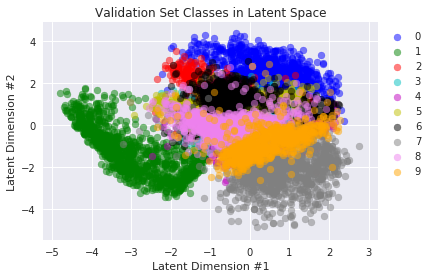
\includegraphics[scale=0.7]{vae1.png}
\end{center} 

Zooming in on the square in this latent space covering $[-2, 2] \times [-2, 2]$, we generate the following corresponding images produced by the decoder.  
 \begin{center}
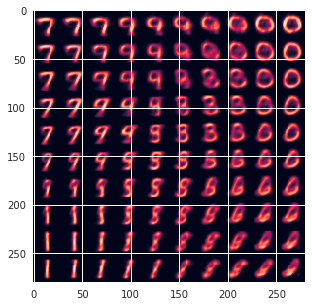
\includegraphics[scale=0.7]{vae2.png}
\end{center} 

We also trained the variational autoencoder with a latent dimension of 20.  Here are images that we generated after training for 200 epochs.  The final training loss is 102.6910 and the final validation loss is 102.6716.  Note that many of these images appear a bit fuzzy -- a known symptom of VAEs. 
 \begin{center}
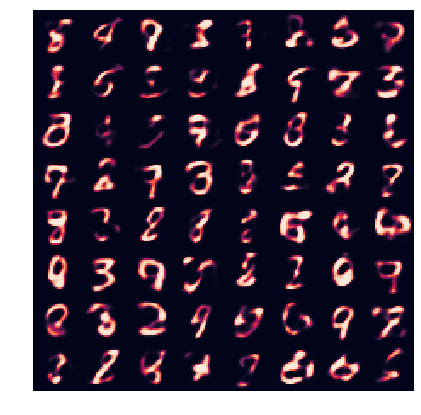
\includegraphics[scale=0.5]{vae3.png}
\end{center} 

We also sampled two latent vectors $z_1, z_2 \sim N(0, I)$ and we plot $x \sim p(x \vert \alpha z_1 + (1 - \alpha) z_2)$ for $\alpha = 0.0, 0.2, 0.4, 0.6, 0.8, 1.0$.
 \begin{center}
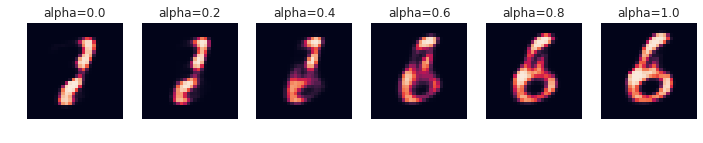
\includegraphics[scale=0.7]{vae4.png}
\end{center} 

\subsection{Generative Adversarial Network} 
We normalize all images to have values between -1 and 1, and de-normalize the generated images for visualization purposes. Our final GAN model consists of a generator and discriminator. The discriminator comprises 2 linear layers with LeakyReLU activations, followed by a linear output layer with Sigmoid activation. The generator comprises 2 linear layers with LeakyReLU activations, followed by a linear output layer with Tanh activation. The hidden dimension size for both $D$ and $G$ is 256. Because the stability of the GAN game suffers when we have sparse gradients, we achieve better results using the LeakyReLU activation (with negative slope 0.2) instead of the ReLU activation.

We train $G$ to maximize $\log(D(G(z))$ instead of minimizing $\log(1-D(G(z)))$ (\cite{gan}). Note that the new form of the loss is functionally equivalent, but enables stronger gradients early in training when the discriminator can be very confident about samples from the generator. During training for GAN's, the discriminator can be trained for $k$ steps before updating the generator once; if the generator is trained ``too much'' without updating the discriminator, it may simply learn to map many values of $x$ to the same $z$ and fail to be expressive enough to capture the latent data distribution. We find that setting $k=1$ is sufficient for our purposes. For both the generator and discriminator, we use the Adam optimizer with learning rate 0.0005 and train the model for 300 epochs.

The input to the generator is a noise vector, which is sampled from a spherical normal prior $p(\mathbf{z}) = \mathcal{N}(\mathbf{0}, \mathbf{I})$.

Because the MNIST dataset also provided labels for the data, we additionally tried improving the model's generator by training the discriminator to also classify the samples. To do this, we implemented an auxillary GAN, which shared the first 2 layers of the generator's neural network, but whose output layer consisted of a linear layer and softmax activation. The results for this modified model appear similar to the original network, and are also shown below.

\begin{figure}[H]
	\begin{center}
		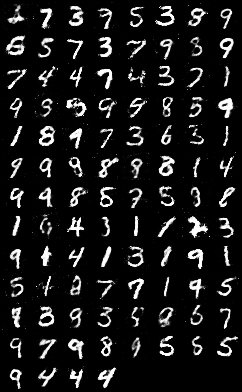
\includegraphics[scale=0.5]{fake_images-200}
		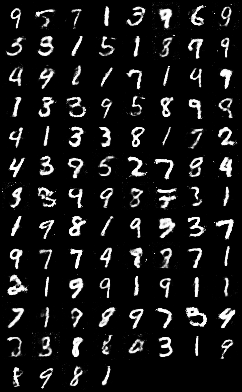
\includegraphics[scale=0.5]{fake_images-200-mod}
		\label{fig:gan-vis}
		\caption{Left: Visualization of 100 generated samples from random noise vectors sampled from a spherical normal prior with dimension 64. Right: 100 samples generated using the modified GAN with auxillary digit classification network.}
	\end{center} 
\end{figure}

\begin{figure}[H]
	\begin{center}
		
\includegraphics[scale=0.5]{interp_fake_images-1}
		
\includegraphics[scale=0.5]{interp_fake_images-2} \\
		
\includegraphics[scale=0.5]{interp_fake_images-1-mod}
		
\includegraphics[scale=0.5]{interp_fake_images-2-mod}
		\label{fig:gan-vis}
		\caption{Top: Visualization of samples generated from interpolations of 2 random noise vectors sampled from a spherical normal prior with dimension 64. Bottom: Interpolated samples generated using GAN with auxiliary network.}
	\end{center} 
\end{figure}

\section{Conclusion}
In this practical, we implemented two models to generate written digit images: A Generative Adverasarial Network and a Variational Autoencoder.


\bibliography{writeup}
\nocite{*}
\bibliographystyle{apalike}

\end{document}
